%!TEX root = TFG.tex

\chapter{Diseño y resolución}

En este capítulo se realiza la descripción de los experimentos realizados, su análisis y la búsqueda de un modelo de Machine Learning, así como los resultados finales del trabajo.

En este trabajo se usará una topología de red como la que ilustra la Fig. \ref{fig:top}. En dicha topología podemos ver que tenemos un observador (modelo RockPro64) y 5 dispositivos a analizar (Raspberry Pi).

\begin{figure}
    \centering
    \resizebox{0.5\textwidth}{!}{
        \begin{tikzpicture}
    \node (1) {
\includegraphics{cisco_icons/cloud}};
    \node (2) [below = of 1] {
\includegraphics{cisco_icons/router}};
    \node (3) [below = of 2] {$\substack{
\includegraphics{cisco_icons/pc} \\ \text{Observador}}$};
    \node (aux) [below =0.4cm of 3] {};
    \node (4) [below = of aux] {$\substack{
\includegraphics{cisco_icons/pc} \\ \text{Disp. 3}}$};
    \node (5) [left = of 4] {$\substack{
\includegraphics{cisco_icons/pc} \\ \text{Disp. 2}}$};
    \node (6) [left = of 5] {$\substack{
\includegraphics{cisco_icons/pc} \\ \text{Disp. 1}}$};
    \node (7) [right = of 4] {$\substack{
\includegraphics{cisco_icons/pc} \\ \text{Disp. 4}}$};
    \node (8) [right = of 7] {$\substack{
\includegraphics{cisco_icons/pc} \\ \text{Disp. 5}}$};
    \node (text) {Internet};
    \draw[-] (1) -- (2); 
    \draw[-] (2) -- (3);
    \draw[-] (3) -- (4);
    \draw[-] (aux.center) -| (6);
    \draw[-] (aux.center) -| (5);
    \draw[-] (aux.center) -| (7);
    \draw[-] (aux.center) -| (8);
\end{tikzpicture}
    }
    \caption{Topología de la red}
    \label{fig:top}
\end{figure}

La idea es mandar mensajes desde el observador a cada uno de los dispositivos y que cada uno de los dispositivos conteste a esos mensajes y podamos obtener una marca de tiempo en ese dispositivo.

\section{Elección del protocolo}

Las opciones barajadas han sido TCP e ICMP. En un principio se pensaba usar las marcas de tiempo contenidas en las cabeceras de estos protocolos, pero esta idea se descartó puesto que únicamente permitían obtener los tiempos en milisegundos. El objetivo era obtener los tiempos en nanosegundos por tanto, se enviaron los datos en el cuerpo del paquete que no tiene una limitación tan corta de espacio. 

Con el fin de mantener la conexión persistente en toda la muestra se escogió el protocolo TCP, ya que una vez establecida la conexión la mantendremos hasta el final.

\section{Obtención de datos}

Para obtener los datos usaremos una estructura cliente-servidor. En nuestro los dispositivos a analizar serán los que tomen el rol de servidores y el observador será el cliente.

Con esta idea en mente creamos un programa servidor que escuche a cualquier dirección IP en un determinado puerto y responda con una marca de tiempo en nanosegundos. Este programa se ejecutará en cada uno de los dispositivos bajo análisis.

A la hora de capturar los datos se usó un reloj interno que no debería sufrir alteraciones que disminuyeran su valor (\texttt{steady\_clock}\cite{steadyclockcpp}).

Una vez los dispositivos estén todos escuchando, el observador ejecutará un programa cliente que es el que se encargará de enviar los mensajes al servidor correspondiente. Este programa guarda una marca de tiempo al comienzo de la ejecución $t_{start}$, que será nuestro punto de referencia. Después mandará $n$ mensajes equiespaciados en intervalos de 1 segundo.

En cada ejecución del bucle se obtendrá una marca de tiempo en el observador $t_i$, y una marca de tiempo del dispositivo $t'_i$. Con esto conseguimos tener varios datos:
\begin{itemize}
    \item La marca de tiempo relativa a cada mensaje desde el inicio, $t_i - t_{start}$. Teóricamente debería de dar valores exactos, ya que se manda un mensaje cada segundo, pero existe cierto retraso.
    \item La marca de tiempo absoluta del observador $t_i$.
    \item La marca de tiempo absoluta del dispositivo $t'_i$.
    \item La desviación del reloj del dispositivo respecto al del observador, $t_i - t'_i$.
\end{itemize}

Un ejemplo de como se guardan estos datos se puede ver en la Tabla \ref{tab:trace_example}.
\begin{table}
    \centering
    \resizebox{0.75\textwidth}{!}{
    \begin{tabular}{c|c|c|c|c}
        \texttt{time} & \texttt{TSrock} & \texttt{TSrasp} & \texttt{offset} & \texttt{device} \\
        \hline\hline
        292 & 119238112796030 & 104592709716803 & -14645403079227 & 192.168.1.111 \\
        1001191222 & 119239113986960 & 104593710167425 & -14645403819535 & 192.168.1.111 \\
        2001485862 & 119240114281600 & 104594710453699 & -14645403827901 & 192.168.1.111 \\
        \vdots & \vdots & \vdots & \vdots & \vdots
    \end{tabular}
    }
    \caption{Ejemplo de los datos obtenidos de cada dispositivo}
    \label{tab:trace_example}
\end{table}

Este proceso se realizará para cada dispositivo tanto en una muestra secuencial, como en una muestra en paralelo.


\section{Análisis de los datos}

En esta sección analizaremos el incremento de la desviación del reloj en cada una de las muestras, así como la desviación acumulada en cada punto.

\subsection{Experimento 1: Muestra secuencial}

En este primer experimento se ha tomado una muestra de \SI{7200}{} segundos, es decir, \SI{2}{} horas por dispositivo, lo que en total suman \SI{10}{} horas de muestras.

En la Fig. \ref{fig:off_acu_secuencial} observamos la desviación (offset) acumulada en cada dispositivo durante esas \SI{2}{} horas.

\begin{figure}
    \centering
    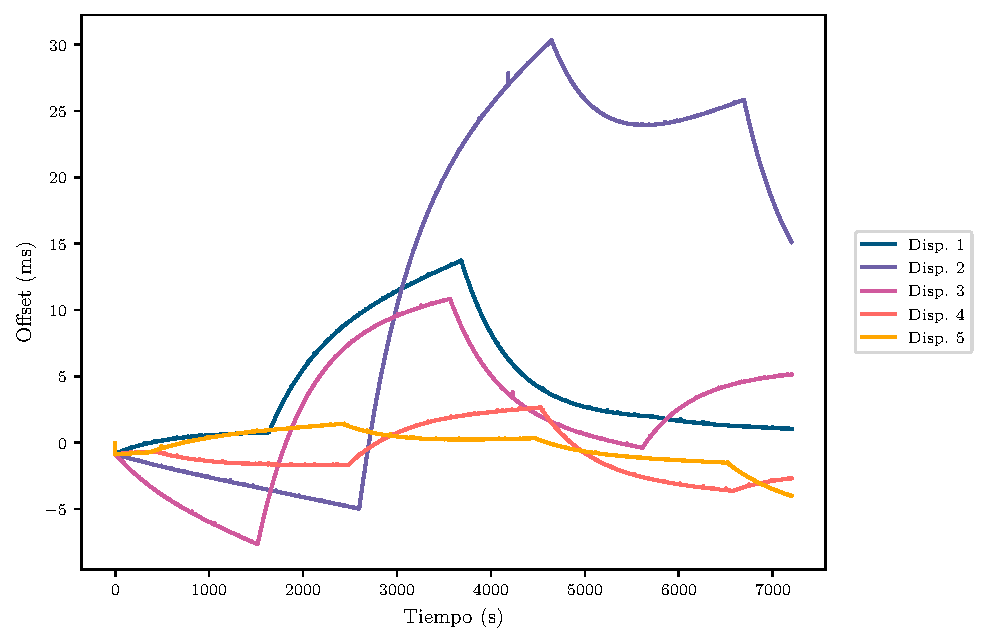
\includegraphics[scale=0.65]{../Python/plots/individual/offset_plot}
    \caption{Offset acumulado muestra secuencial}
    \label{fig:off_acu_secuencial}
\end{figure}

Como se puede ver hay 2 tipos de comportamiento. Los dispositivos 1, 2 y 3 se mantienen monótonos al comienzo para después incrementar mucho su desviación. Por contra los dispositivos 4 y 5 se mantienen sin grandes cambios en toda la muestra. Esto se puede ver más claramente en la Fig. \ref{fig:off_acu_secuencial_diffs}.

\begin{figure}
    \centering
    \subfloat[Dispositivos 1, 2 y 3]{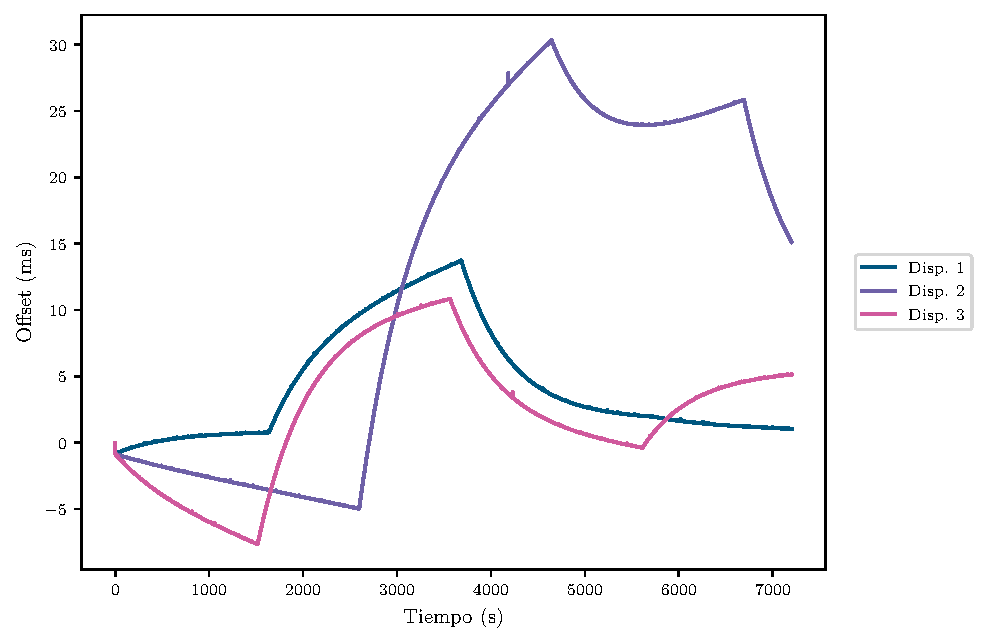
\includegraphics[width=0.4\textwidth]{../Python/plots/individual/offset_plot_123}}
    \quad
    \subfloat[Dispositivos 4 y 5]{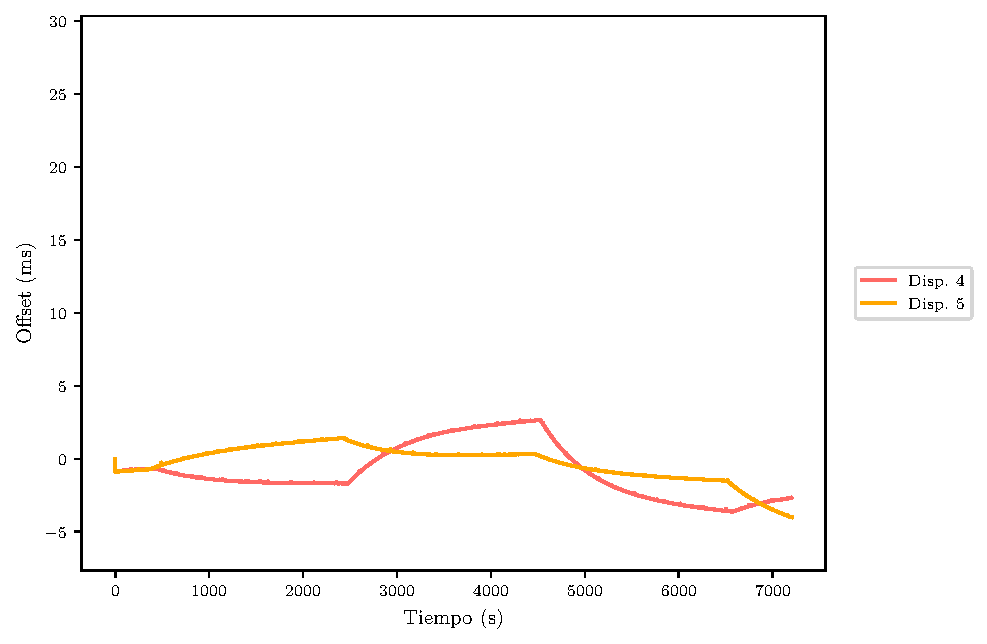
\includegraphics[width=0.4\textwidth]{../Python/plots/individual/offset_plot_45}}
    \caption{Diferencias entre offsets de dispositivos}
    \label{fig:off_acu_secuencial_diffs}
\end{figure}

Lo que nos interesa al final es obtener una forma de distinguir estadísticamente los datos, para ello podemos generar un gráfico que nos muestre entre que valores se mueven estos datos en cada dispositivo, en definitiva, lo podemos ver con diagrama de cajas (Fig. \ref{fig:box_secuencial}). Se han eliminado los valores atípicos ya que a tan pequeña escala no dejan ver los verdaderos resultados.

\begin{figure}
    \centering
    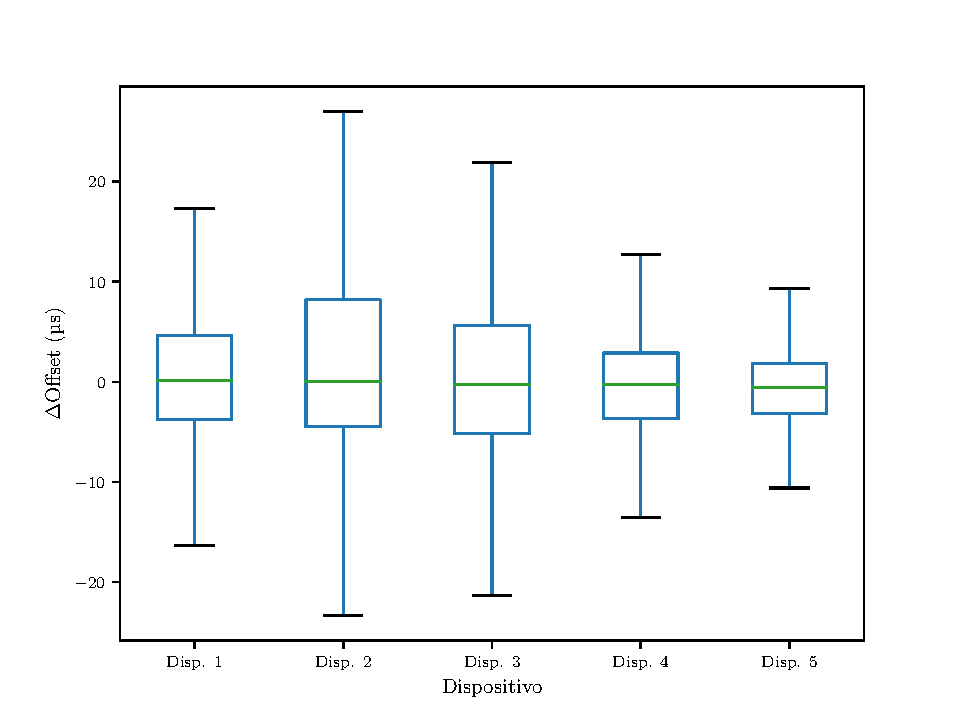
\includegraphics[scale=0.7]{../Python/plots/individual/boxplot_no_out}
    \caption{Diagrama de cajas muestra secuencial}
    \label{fig:box_secuencial}
\end{figure}

Con este diagrama podemos ver lo comentado anteriormente. Los dispositivos 4 y 5 son los que menos varían, esto se puede ver en que las cajas son pequeñas y la mediana está centrada entre los cuartiles (Q1 y Q3). 

En los otros 3 dispositivos vemos como entre la mediana y el tercer cuartil hay más espacio que entre la mediana y el primer cuartil. Esto se debe a que tienen muchos incrementos grandes, por eso crecen tan bruscamente.

Con esto nos hacemos una idea de los dispositivos son distinguibles estadísticamente, lo que nos confirma que podremos entrenar un modelo que los identifique.

\iffalse
Por último obtenemos las variables estadísticas que podrán ser usados para entrenar los modelos (Tabla \ref{tab:stats_sec}). 

\begin{table}
    \centering
    \resizebox{0.85\textwidth}{!}{
        \begin{tabular}{c|c|c|c|c|c|c|c|c|c|c|c}
             & Sum & Mean & Median & Mode & Std & IQR & Kurtosis & Skew & Max & Min & Device \\
             \hline\hline
            1 & 161935.0 & 2698.9166666666665 & 2368.0 & -10638.0 & 4811.992019561929 & 4723.75 & 1.9261137847830017 & 0.393744697396757 & 16643.0 & -10638.0 & Disp. 1 \\
            2 & -133618.0 & -2226.9666666666667 & -2069.0 & -14962.0 & 4940.972387543091 & 3037.75 & 3.06918010272503 & 0.3990191392522864 & 12839.0 & -14962.0 & Disp. 2 \\
            3 & -474582.0 & -7909.7 & -8169.5 & -21129.0 & 4835.756096735922 & 4555.0 & 3.6509891533583105 & 0.7015937932968024 & 10047.0 & -21129.0 & Disp. 3 \\
            4 & 38723.0 & 645.3833333333333 & 343.5 & -511.0 & 2546.367949044463 & 2792.25 & 1.237821148508425 & 0.6920187401340381 & 8323.0 & -4649.0 & Disp. 4 \\
            5 & 18048.0 & 300.8 & 221.5 & -8231.0 & 3895.818561535789 & 4542.0 & 0.10736681592393049 & 0.13881288039853917 & 9109.0 & -8231.0 & Disp. 5 \\
            6 & 155944.0 & 2599.0666666666666 & 2368.0 & -10638.0 & 4960.2799021168785 & 4723.75 & 1.6897518199182318 & 0.28091999994143674 & 16643.0 & -10638.0 & Disp. 1 \\
            \vdots & \vdots & \vdots & \vdots & \vdots & \vdots & \vdots & \vdots & \vdots & \vdots & \vdots & \vdots \\
        \end{tabular}
    }
    \caption{Datos estadísticos muestra secuencial}
    \label{tab:stats_sec}
\end{table}
\fi


\subsection{Experimento 2: Muestra paralela}

Para el segundo experimento se han capturado datos de todos los dispositivos simultáneamente durante un periodo de \SI{43200}{} segundos, es decir, \SI{12}{} horas.

En la Fig. \ref{fig:off_acu_paralelo} podemos ver la desviación acumulada en cada dispositivo en este periodo de tiempo. En este gráfico también se han marcado ciertos puntos en los que los dispositivos parecen ``sincronizarse''. Con esto nos referimos a que alrededor de estas marcas de tiempo todos los dispositivos cambian de tendencia bruscamente y además parecen repetirse con cierta periodicidad. Las marcas de tiempo de este gráfico corresponden a los puntos $\{\SI{4000}{},  \SI{16500}{}, \SI{29000}{}, \SI{41000}{}\}$ que están aproximadamente equidistantes (aproximadamente \SI{12000}{} segundos).

\begin{figure}
    \centering
    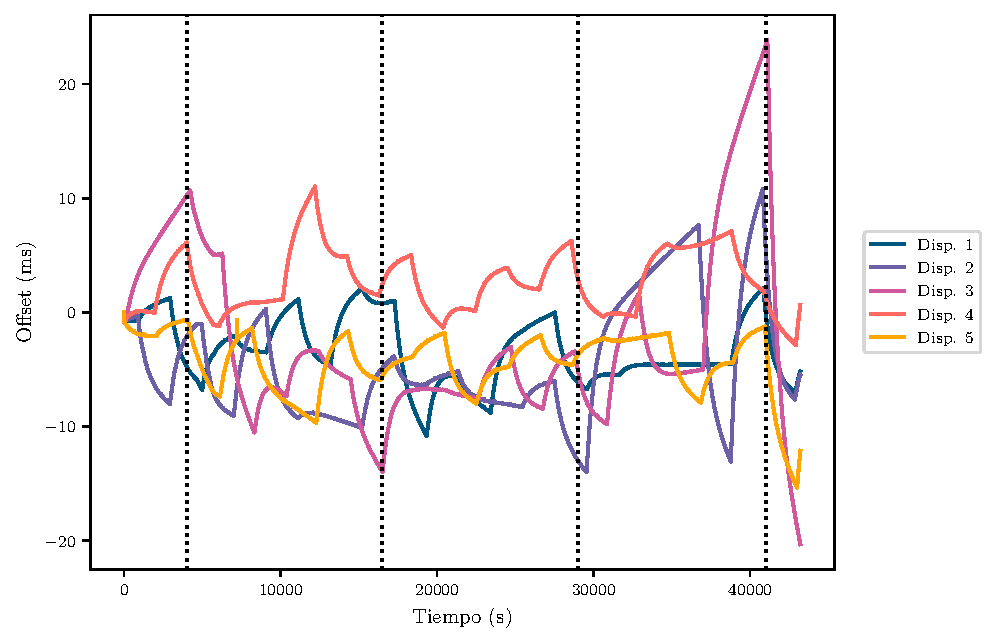
\includegraphics[scale=0.65]{../Python/plots/parallel/offset_plot}
    \caption{Offset acumulado muestra paralela}
    \label{fig:off_acu_paralelo}
\end{figure}

Esta ``sincronización'' entre dispositivos parece deberse a algún tipo de actualización del reloj interno del dispositivo mediante algún demonio del sistema operativo. El principal demonio que se encarga de esta tarea es el servicio NTP, el cual fue desactivado para realizar estas pruebas. 

Si consultamos otro diagrama de cajas con el incremento de la desviación en cada instante (Fig. \ref{fig:box_paralelo}) podemos ver como todos los dispositivos están mucho a la par que en la muestra secuencial (Fig. \ref{fig:box_secuencial}).  Siguen teniendo ciertas diferencias, por lo cual concluimos que son estadísticamente diferenciables también.

\begin{figure}
    \centering
    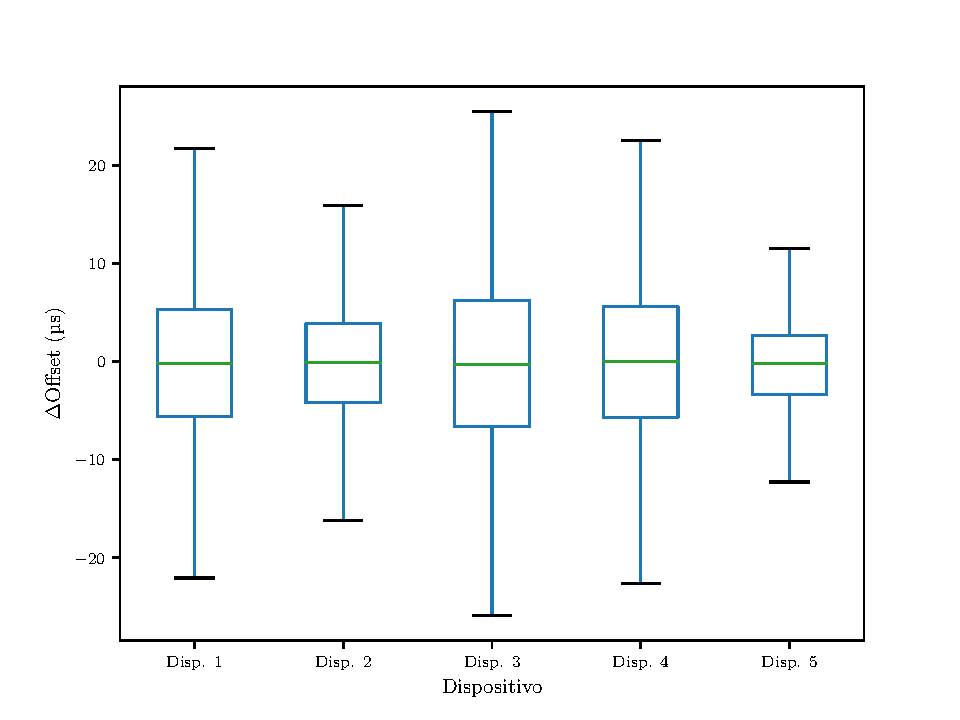
\includegraphics[scale=0.7]{../Python/plots/parallel/boxplot_no_out}
    \caption{Diagrama de cajas muestra paralela}
    \label{fig:box_paralelo}
\end{figure}

\section{Elección de la muestra de datos}

Analizando los incrementos de la desviación en ambas muestras vemos que la muestra paralela tiene valores más parecidos a los que esperaríamos. Estos valores de incremento de la desviación son más pequeños y más parecidos entre todos los dispositivos, es por ello que entrenaremos los modelos con los datos de la muestra paralela.

Estos datos se obtendrán mediante una ventana deslizante de \SI{1}{} minuto sobre el incremento de la desviación del reloj del dispositivo. Usaremos las siguientes variables estadísticas:
\begin{multicols}{2}
    \begin{itemize}
        \item Suma
        \item Media
        \item Mediana
        \item Moda
        \item Desviación típica
        \item Rango intercuartílico
        \item Curtosis
        \item Coeficiente de asimetría (skewness)
        \item Máximo
        \item Mínimo
    \end{itemize}
\end{multicols}

Generando estos datos estadísticos de la muestra paralela mediante la ventana deslizante, obtenemos los resultados que se pueden ver en la Tabla \ref{tab:stats_par}. Estos datos estadísticos serán los que posteriormente se usarán para entrenar un modelo de Machine Learning.

\begin{table}
    \centering
    \resizebox{0.85\textwidth}{!}{
        \begin{tabular}{c|c|c|c|c|c|c|c|c|c|c|c}
             & Sum & Mean & Median & Mode & Std & IQR & Kurtosis & Skew & Max & Min & Device \\
            \hline\hline
            1 & 21773.0 & 362.8833333333333 & -306.5 & -17885.0 & 8212.584818005707 & 12095.5 & 0.0567239505757037 & 0.4351150677774124 & 20799.0 & -17885.0 & Disp. 1 \\
            2 & 4059.0 & 67.65 & 239.5 & -15862.0 & 5615.809629134339 & 3012.25 & 1.400480680742287 & -0.1242668154207108 & 14194.0 & -15862.0 & Disp. 2 \\
            3 & 1187.0 & 19.78333333333333 & 503.5 & -25009.0 & 7760.832728977938 & 8467.0 & 1.231550787741679 & -0.2621794660161829 & 20510.0 & -25009.0 & Disp. 3 \\
            4 & 74154.0 & 1235.9 & 2016.5 & -21616.0 & 8391.731753359314 & 9663.75 & 0.4104874852336051 & -0.4087239664161064 & 19992.0 & -21616.0 & Disp. 4 \\
            5 & -127078.0 & -2117.9666666666667 & -2385.0 & -11894.0 & 4354.015072678016 & 2737.0 & 1.9665757630194 & 0.6070065306393123 & 10383.0 & -11894.0 & Disp. 5 \\
            6 & 20147.0 & 335.78333333333336 & -306.5 & -17885.0 & 8244.497450208664 & 12095.5 & 0.0362682762350909 & 0.4263535051366743 & 20799.0 & -17885.0 & Disp. 1 \\
            \vdots & \vdots & \vdots & \vdots & \vdots & \vdots & \vdots & \vdots & \vdots & \vdots & \vdots & \vdots \\
        \end{tabular}
    }
    \caption{Datos estadísticos muestra paralela}
    \label{tab:stats_par}
\end{table}

\section{Reducción de la dimensionalidad}

En esta sección buscaremos valores estadísticos correlacionados entre sí. En caso de existir habrá que eliminarlos antes de entrenar los modelos, puesto que no aportan información y provocarán que el algoritmo tarde aún más tiempo en ser entrenado.

La correlación entre las variables estadísticas se puede ver en la Fig. \ref{fig:corr}. Vemos como suma, media y mediana son las variables más correlacionadas entre sí, por tanto serán eliminadas 2 de ellas.

\begin{figure}
    \centering
    \subfloat[Correlación entre las variables iniciales]{
        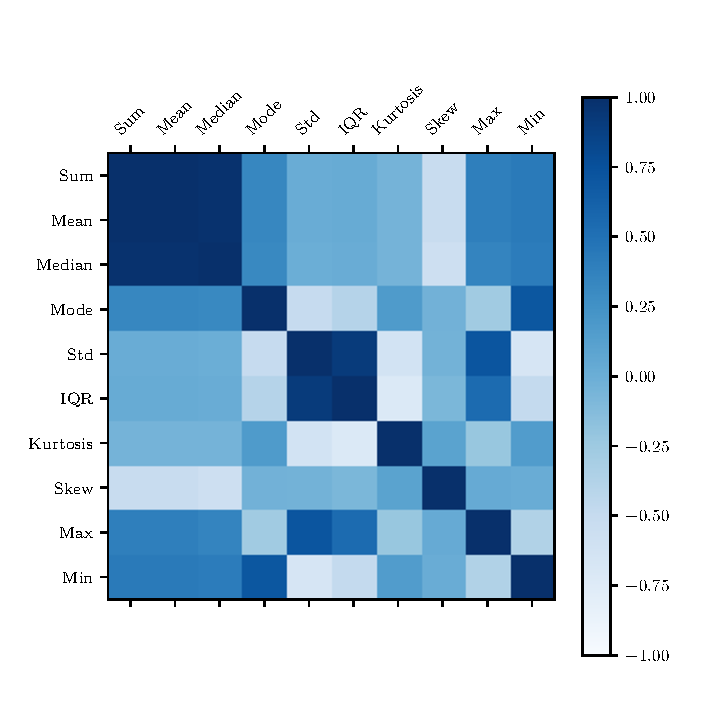
\includegraphics[scale=0.55]{../Python/plots/parallel/correlacion_stats.pdf}
    }
    \subfloat[Correlación entre las variables finales]{
        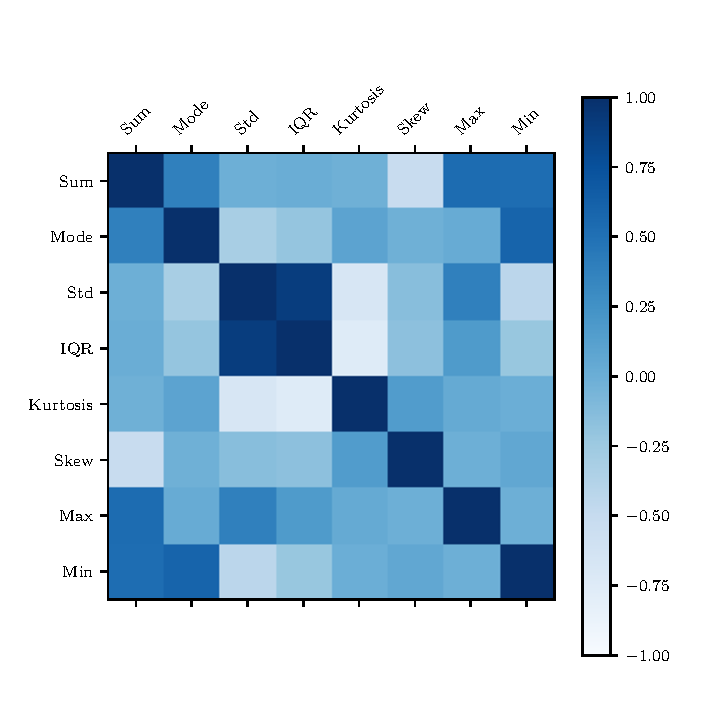
\includegraphics[scale=0.55]{../Python/plots/parallel/correlacion_stats_ftred.pdf}
    }
    \caption{Correlación entre las variables estadísticas}
    \label{fig:corr}
\end{figure} 



\section{Entrenamiento de los modelos}

En esta sección analizaremos los resultados que hemos obtenido de los modelos sobre los datos de la muestra paralela, como hemos concluido en la sección anterior.

Para realizar este entrenamiento se ha usado la librería \texttt{scikit-learn} sobre el lenguaje de programación Python. Esta librería tiene clases que implementan los algoritmos vistos anteriormente que serán los que usemos (Sec. \ref{sec:algorithms}). Las clases que corresponden a cada modelo son las que se ven en la Tabla \ref{tab:equiv_models}.

\begin{table}
    \centering
    \begin{tabular}{c|c}
        Algoritmo & Implementación \\
        \hline\hline
        Árboles de decisión & \texttt{DecisionTreeClassifier} \cite{scikittrees} \\
        Random Forest & \texttt{RandomForestClassifier} \cite{scikitforest} \\
        MLP & \texttt{MLPClassifier} \cite{scikitmlp} \\
        Naive Bayes & \texttt{GaussianNB} \cite{scikitnaivebayes} \\
        KNN & \texttt{KNeighborsClassifier} \cite{scikitknn} \\
        SVM & \texttt{LinearSVC} \cite{scikitsvm}
    \end{tabular}
    \caption{Equivalencia entre algoritmo e implementación}
    \label{tab:equiv_models}
\end{table}

\begin{figure}
    \centering
    \resizebox{0.5\textwidth}{!}{
    \begin{tikzpicture}
        \node[database,label=below:Datos,database radius=1cm,database segment height=0.5cm] (data) {};
        \node (aux) [right = of data] {};
        \node[database,label=below:Entrenamiento,database radius=0.75cm,database segment height=0.375cm] (train) [above right = 2cm of aux] {};
        \node[database,label=below:Test,database radius=0.75cm,database segment height=0.375cm] (test) [below right = 2cm of aux] {};
        \node[database,label=below:{$\underset{\text{Reducido}}{\text{Entrenamiento}}$},database radius=0.5cm,database segment height=0.25cm] (train2) [right = 3cm of train] {};
        \node (aux2) [right = of train2] {};
        \node[database,label=below:Entrenamiento,label=right:70\%,database radius=0.5cm,database segment height=0.25cm] (train3) [above right = of aux2] {};
        \node[database,label=below:Validación,label=right:30\%,database radius=0.5cm,database segment height=0.25cm] (test) [below right = of aux2] {};
        \draw[-] (1.2,0) -- (aux.center);
        \draw[-] (aux.center) |- (3.4, 2.4) node [above, pos=0.75] {70\%};
        \draw[-] (aux.center) |- (3.4, -2.45) node [below, pos=0.75] {30\%};
        \draw[-] (5.5, 2.4) -- (8, 2.4) node [midway, above] {35\%};
        \draw[-] (9.5, 2.4) -- (aux2.center);
        \draw[-] (aux2.center) |- (11.3, 4.1);
        \draw[-] (aux2.center) |- (11.3, 0.66);
    \end{tikzpicture}
    }
    \caption{Particiones de los datos}
    \label{fig:database}
\end{figure}

A la hora de entrenar modelos de machine learning lo primero que debemos hacer es ajustar sus hiperparámetros. Los hiperparámetros de un modelo son parámetros del mismo que se pueden modificar para que este se adapte mejor a los datos con los que se está trabajando o para cambiar la forma en la aprende este modelo también para adaptarse a estos datos.

Tanto para ajustar los hiperparámetros no se usa la completitud de los datos, se usa un modelo entrenamiento/validación/test. Los datos se han dividido en un conjunto de entrenamiento y otro de test, 70\% para entrenamiento y 30\% para test, lo habitual es tener en torno a una tercera parte de los datos para entrenamiento y el resto para test. Este proceso (Fig. \ref{fig:database}) se hace para comprobar la capacidad de generalización del modelo con datos que no haya visto nunca.

Para particionar los datos lo haremos tomando muestras aleatorias, pero ordenadas para mantener la correlación temporal de los datos. Por ejemplo, si tuviéramos los datos $x_1, \dots, x_{20}$, una muestra aleatoria podría ser $x_{15}, x_8, x_3, x_{17}, x_5, x_{12}$ pero si estos datos presentan una correlación temporal, como es nuestro caso, esta se pierde. Por tanto, reordenamos los datos a su orden natural $x_3, x_5, x_8, x_{12}, x_{15}, x_{17}$. 

El conjunto de entrenamiento se usará únicamente con el modelo final y con los hiperparámetros ya ajustados, puesto que contiene una gran cantidad de datos. Para ajustar los hiperparámetros de cada modelo y comparar los modelos entre sí usaremos un conjunto reducido de este, un 35\% de los datos de entrenamiento.

A este subconjunto de los datos de entrenamiento también será dividido en un conjunto de entrenamiento/test, aunque en este caso al conjunto test lo llamaremos conjunto de validación. Con estos conjuntos entrenaremos los algoritmos para ajustar los hiperparámetros y decidir el modelo.

Para comprobar qué hiperparámetros son los que mejor se ajustan se usará la función \texttt{GridSearchCV} \cite{scikitgrid} que nos permite dados un algoritmo y un conjunto de valores para los hiperparámetros probar todas las combinaciones y obtener así un accuracy de cada uno, con lo que podremos compararlos y quedarnos con los mejores. Esta función nos permite usar validación cruzada. La validación cruzada 

Vamos a ajustar los hiperparámetros de un modelo como ejemplo, en este caso elegiremos el algoritmo de Random Forest sobre los datos la muestra paralela. Los hiperparámetros que se ha decido ajustar son:
\begin{itemize}
    \item \texttt{criterion}: función que mide la pureza de los nodos hijos.
    \item \texttt{max\_features}: número de características que se tienen en cuenta para realizar la división de un nodo.
    \item \texttt{n\_estimators}: número de árboles de decisión que participan en el algoritmo.
\end{itemize}

Para evitar que una rama entre en un bucle infinito devido a que no es capaz de dividir correctamente los nodos se ha fijado la profundidad máxima de cada rama (hiperpárametro \texttt{max\_depth}) a un valor de 1000. 

Si nos fijamos primero en los hiperparámetros \texttt{criterion} y \texttt{max\_features} (Fig. \ref{fig:comp_hiperparam1}) vemos que en promedio el mejor valor de \texttt{criterion} es \texttt{gini}. Fijaremos este parámetro y compararemos la totalidad de los valores entre \texttt{max\_features} y \texttt{n\_estimators} (Fig. \ref{fig:comp_hiperparam2}).

\begin{figure}
    \centering
    \subfloat[]{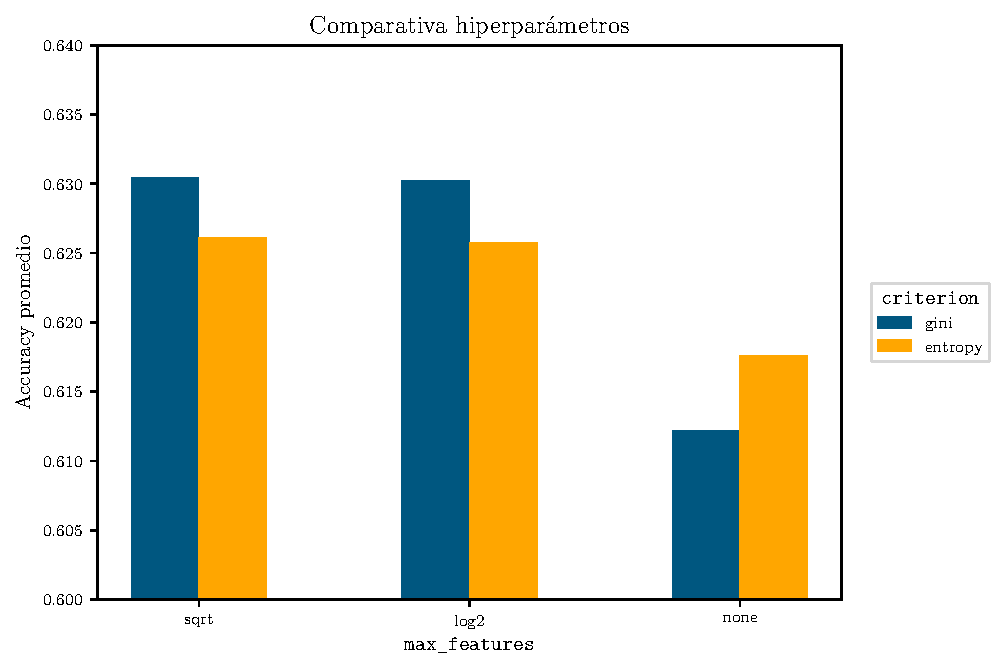
\includegraphics[width=0.45\textwidth]{../Python/plots/parallel/delta_random_forest_results}\label{fig:comp_hiperparam1}}
    \quad
    \subfloat[]{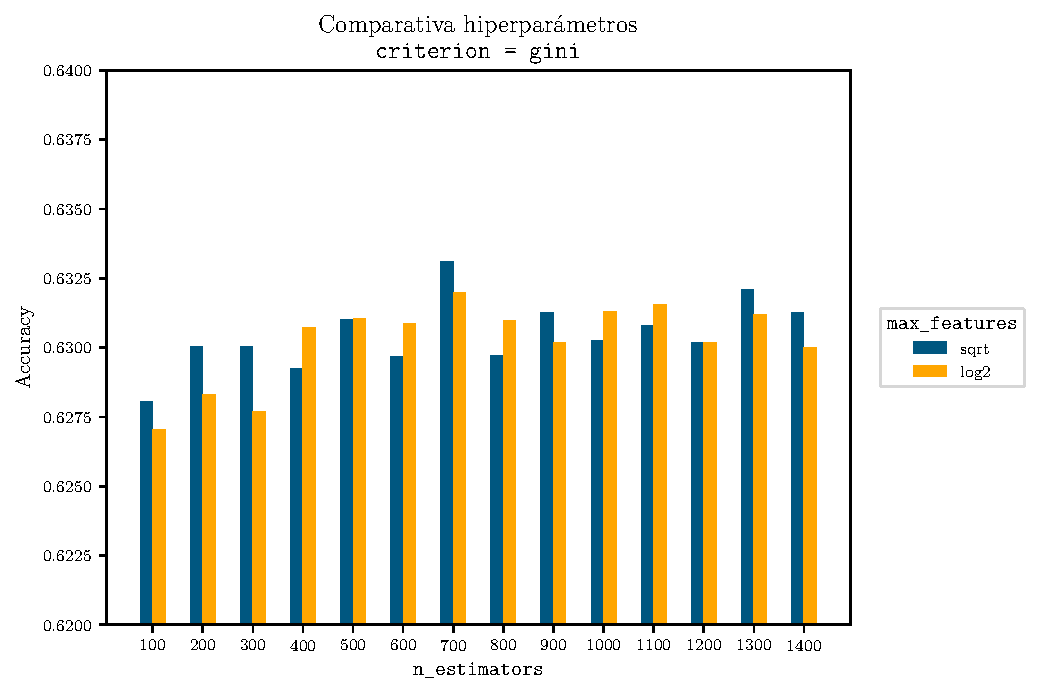
\includegraphics[width=0.45\textwidth]{../Python/plots/parallel/delta_random_forest_results2}\label{fig:comp_hiperparam2}}
    \caption{Comparativa hiperparámetros Random Forest}
    \label{fig:comp_hiperparam}
\end{figure}

En este caso vemos que los mejores valores son \texttt{criterion = gini}, \texttt{n\_estimators = 700} y \texttt{max\_features = sqrt}. Con estos hiperparámetros entrenamos un modelo sobre el conjunto de entrenamiento menor y después realizamos una predicción con el conjunto de validación.

Una vez entrenados todos los modelos con sus mejores hiperparámetros y con un valor de generalización obtenido de la predicción tenemos los resultados que se pueden ver en la Fig. \ref{fig:comp_accur}.

\begin{figure}
    \centering
    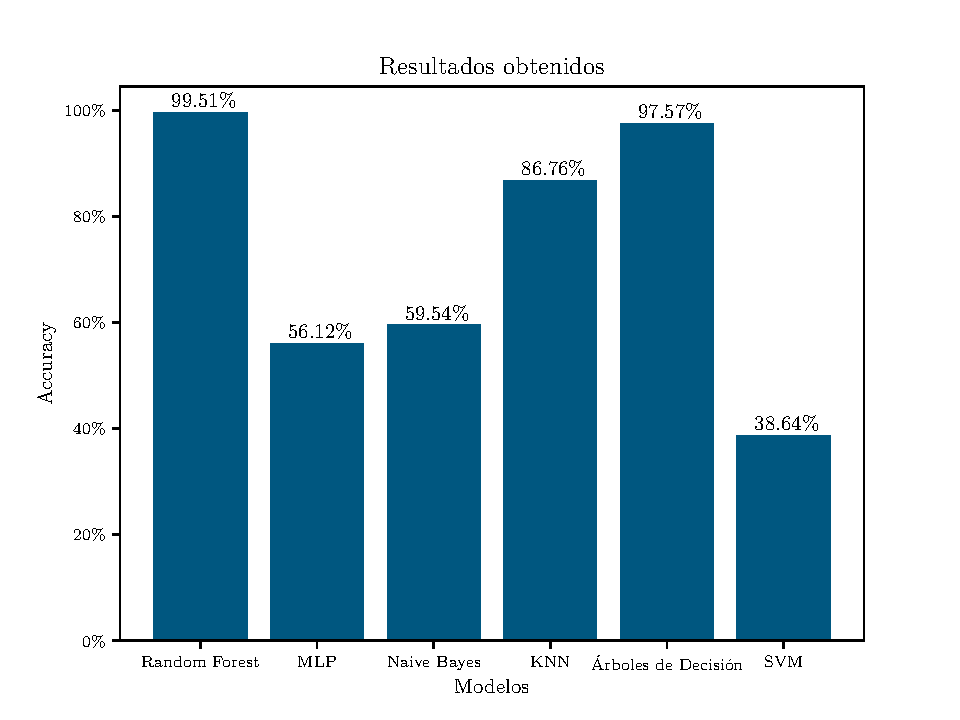
\includegraphics[width=0.4\textwidth]{../Python/plots/parallel/accur_results}
    \caption{Comparativa de resultados entre modelos}
    \label{fig:comp_accur}
\end{figure}

Como se puede ver en ambas muestras los modelos que presentan mejores resultados son los que se basan en árboles de decisión, que son el propio algoritmo de árboles de decisión y random forest. Otra forma de ver estos resultados es mediante las matrices de confusión que nos genera cada algoritmo.

\begin{figure}
    \centering
    \begin{tabular}{ccc}
        \subfloat{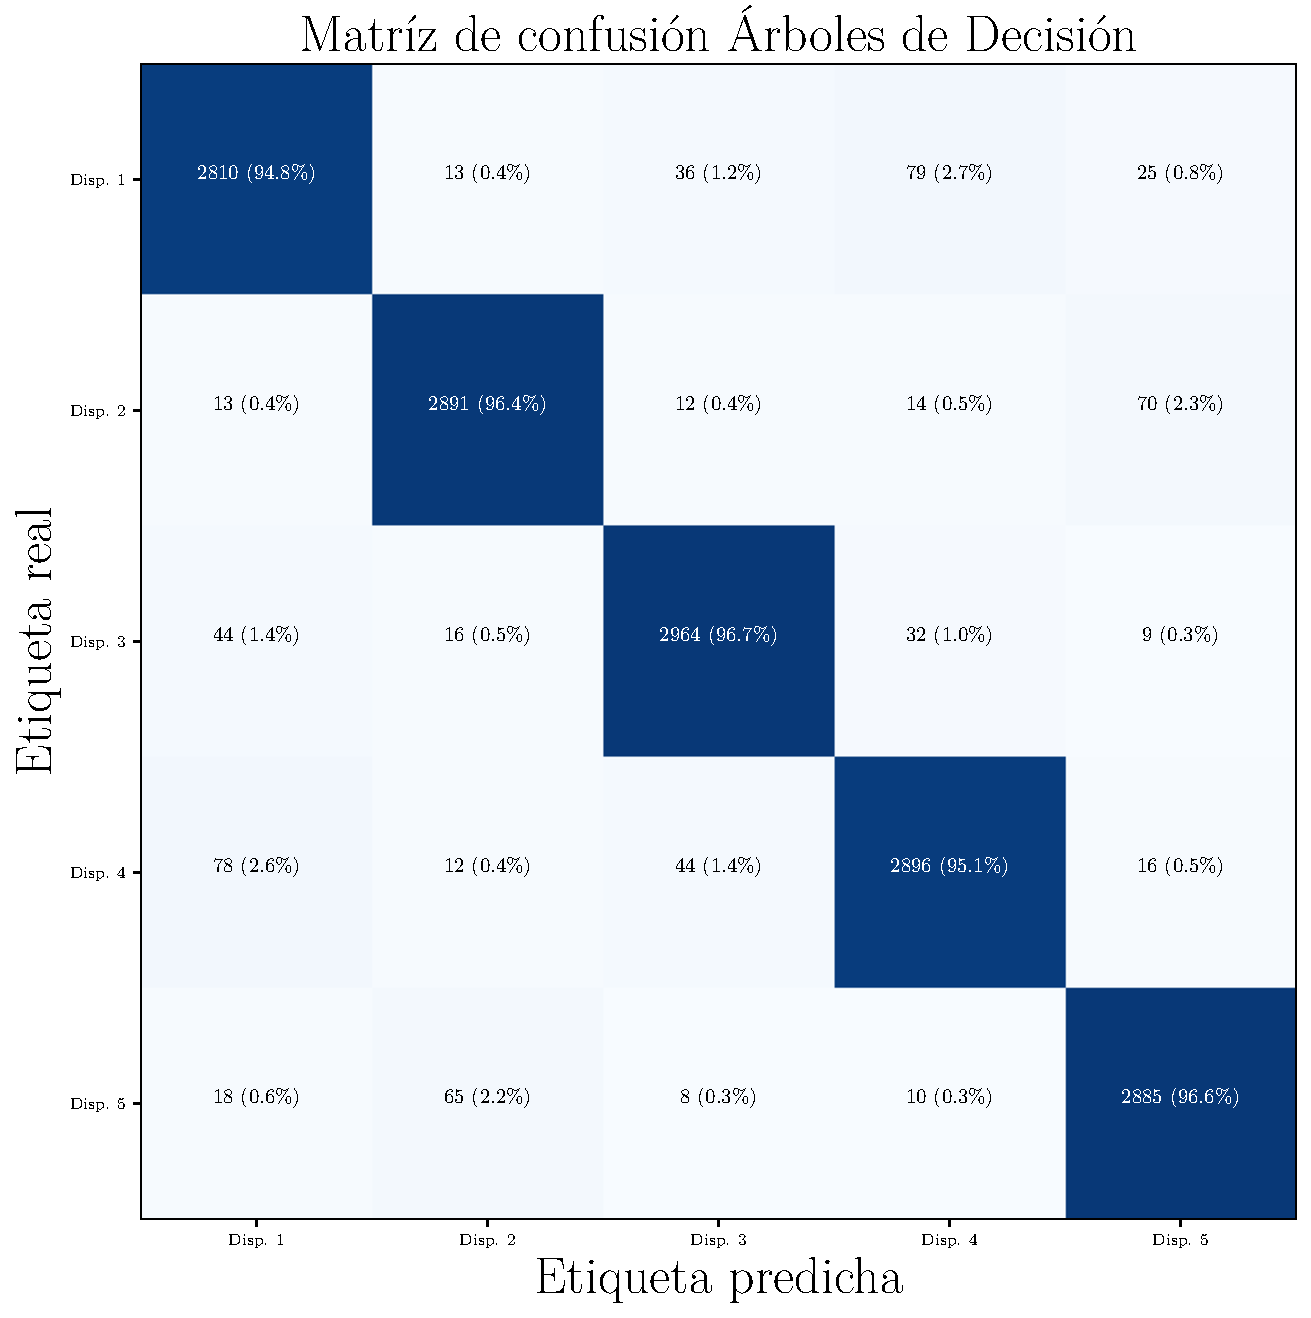
\includegraphics[width=0.4\textwidth]{../Python/plots/parallel/decision_tree_matrix}} & \subfloat{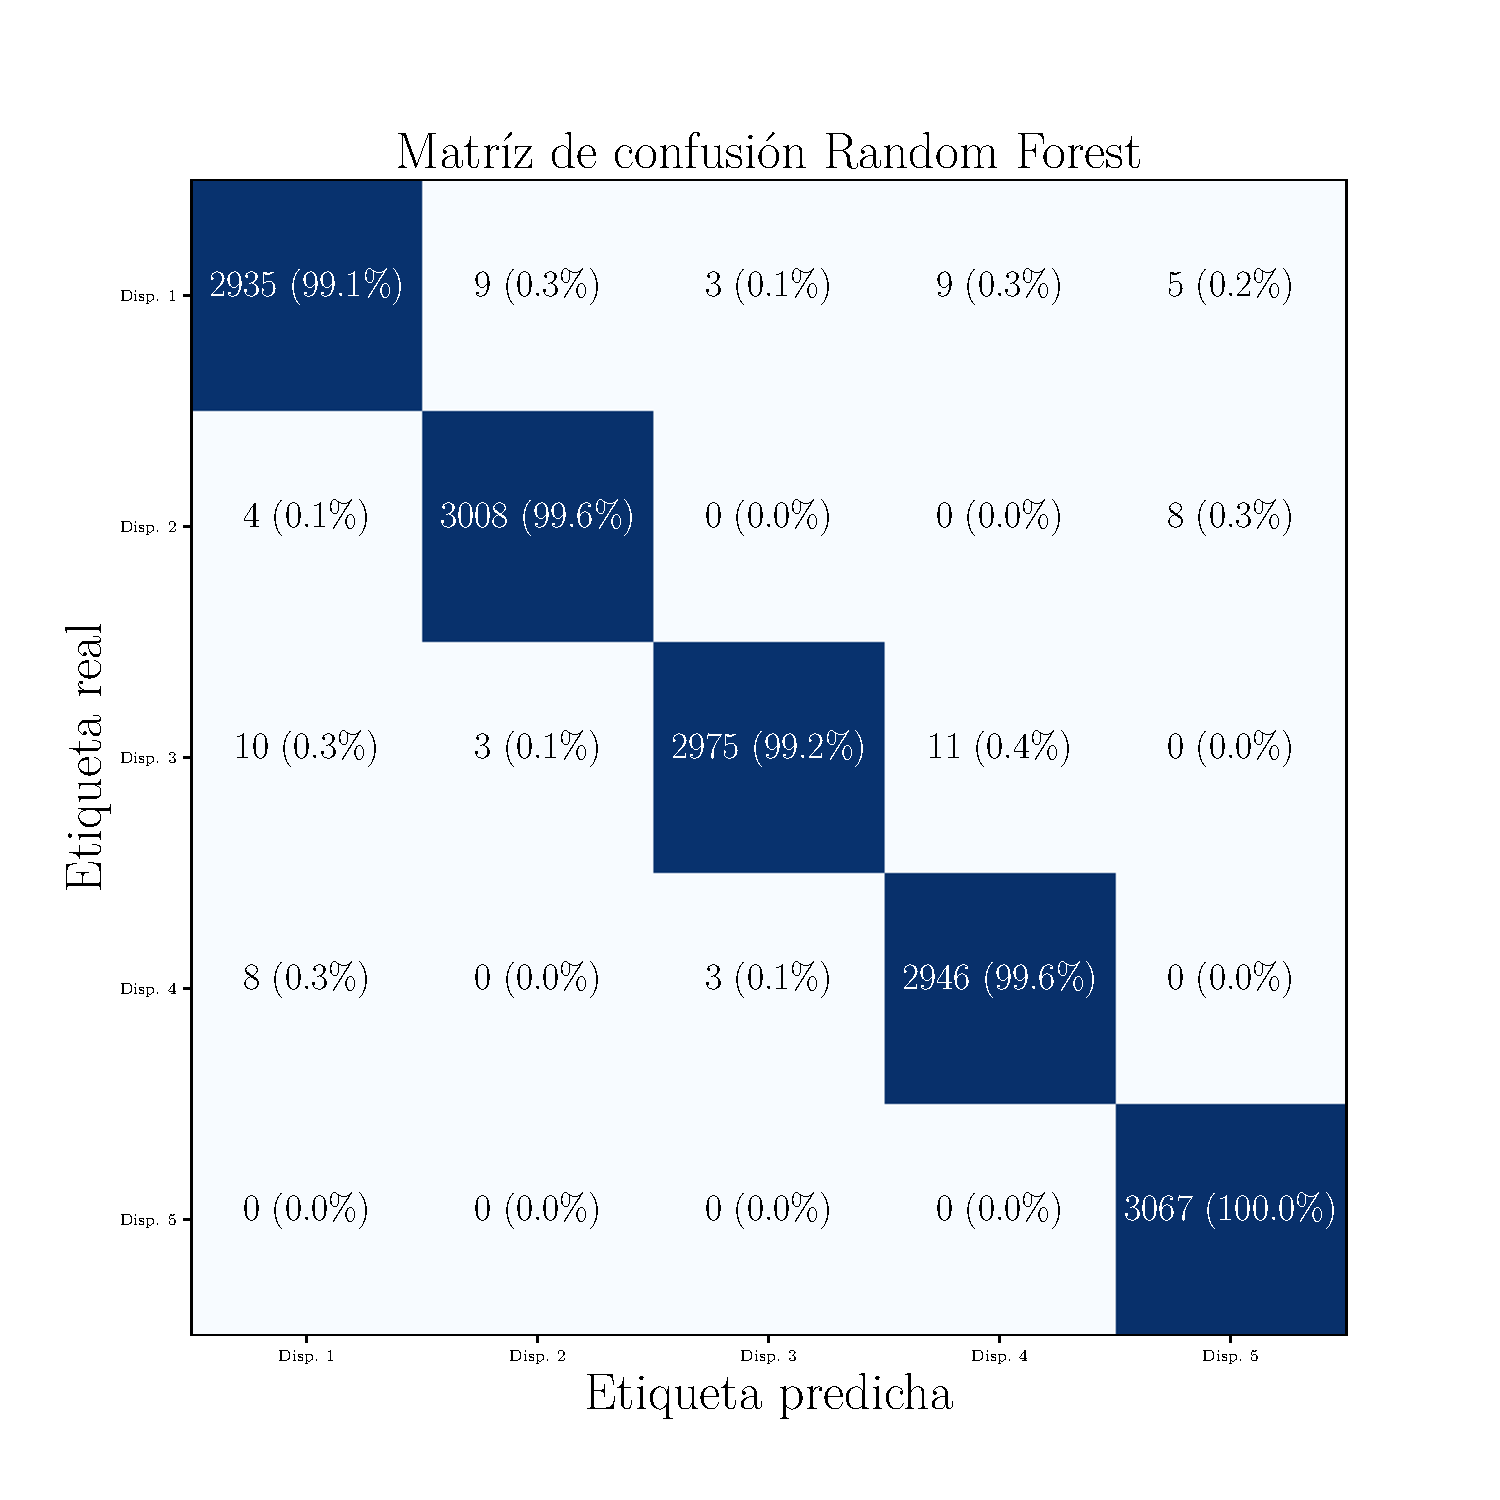
\includegraphics[width=0.4\textwidth]{../Python/plots/parallel/random_forest_matrix}} & \multirow{3}{*}[8em]{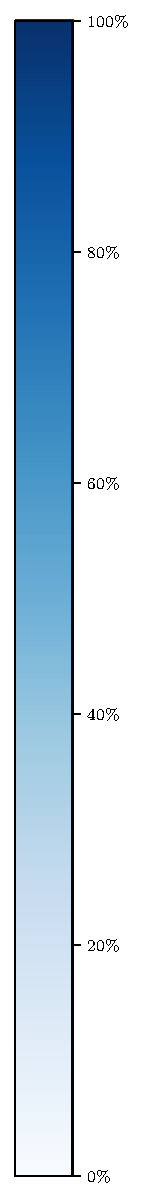
\includegraphics[scale=0.75]{../Python/plots/parallel/colorbar_matrices}} \\
        \subfloat{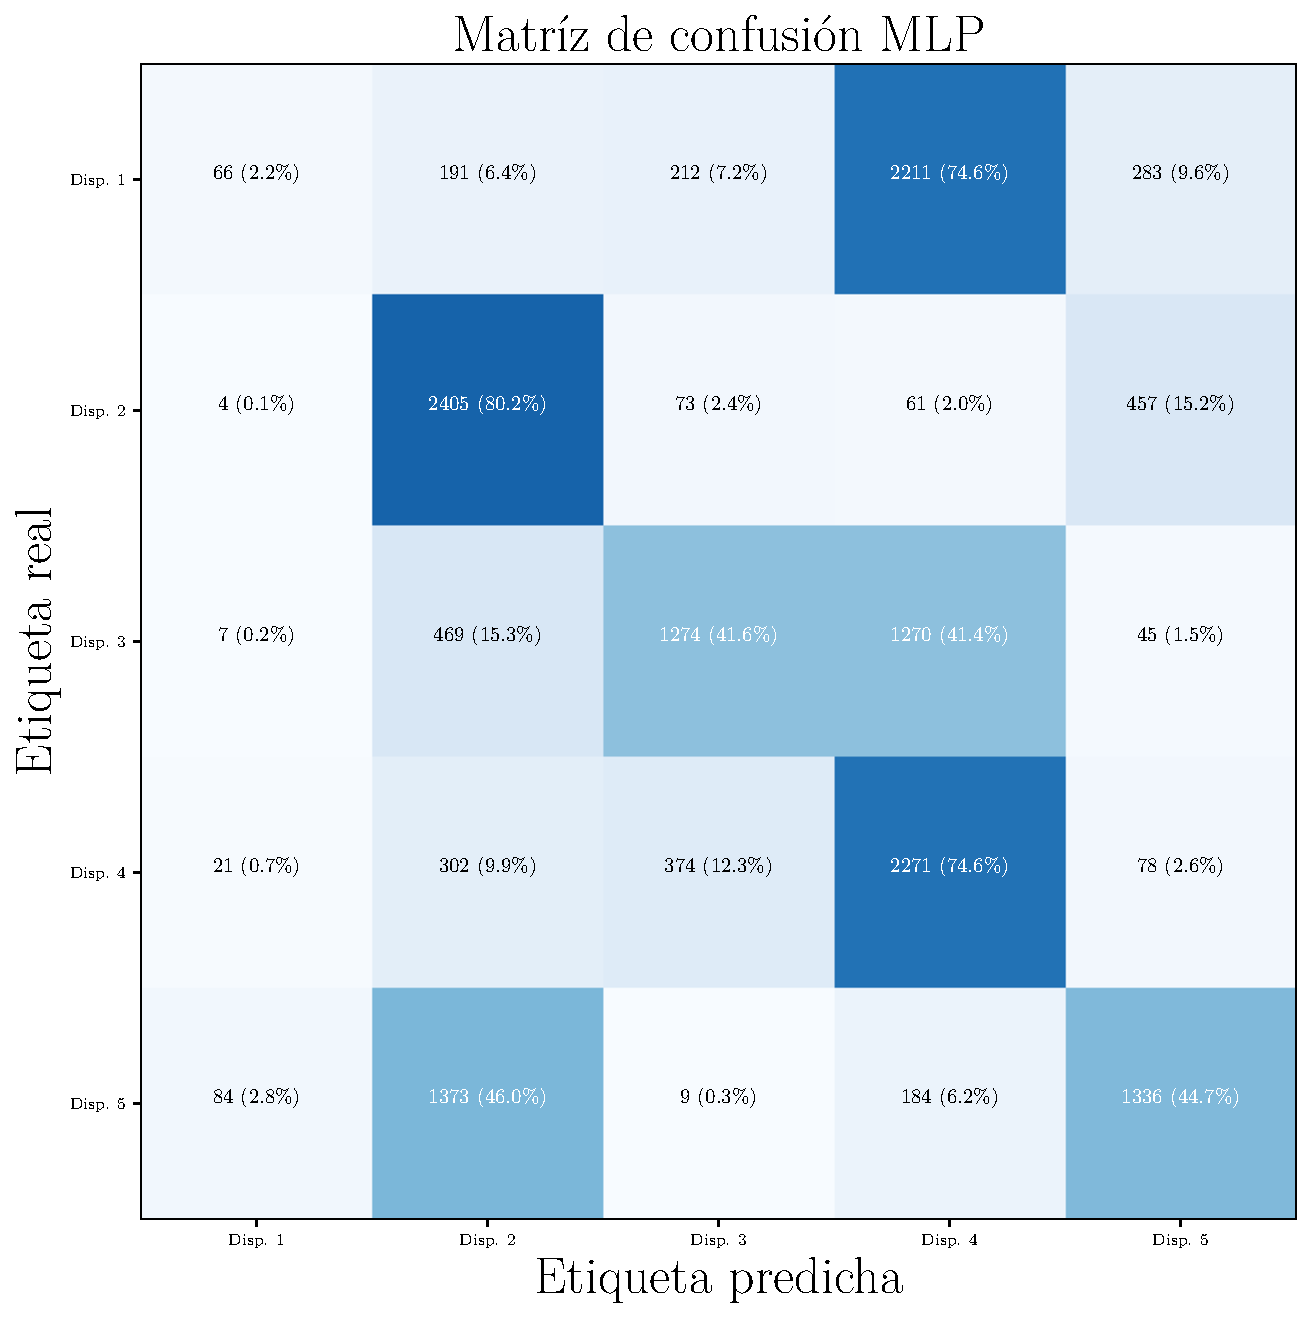
\includegraphics[width=0.4\textwidth]{../Python/plots/parallel/mlp_matrix}} & \subfloat{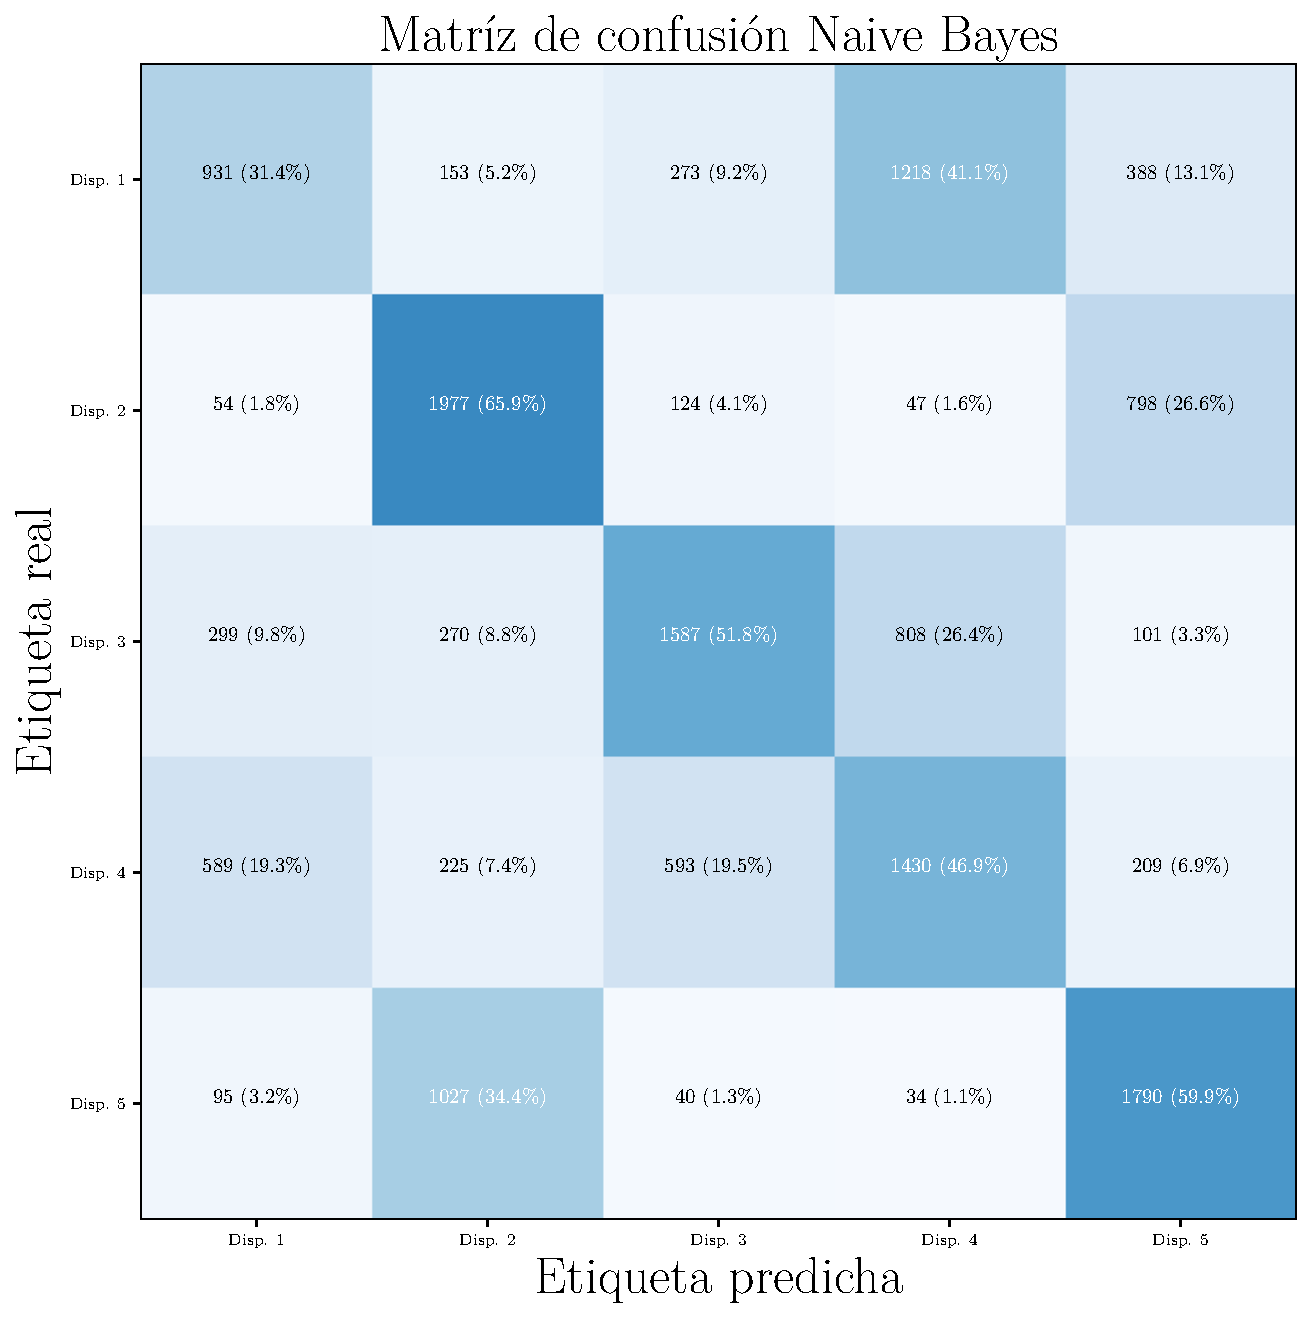
\includegraphics[width=0.4\textwidth]{../Python/plots/parallel/naive_bayes_matrix}} &  \\
        \subfloat{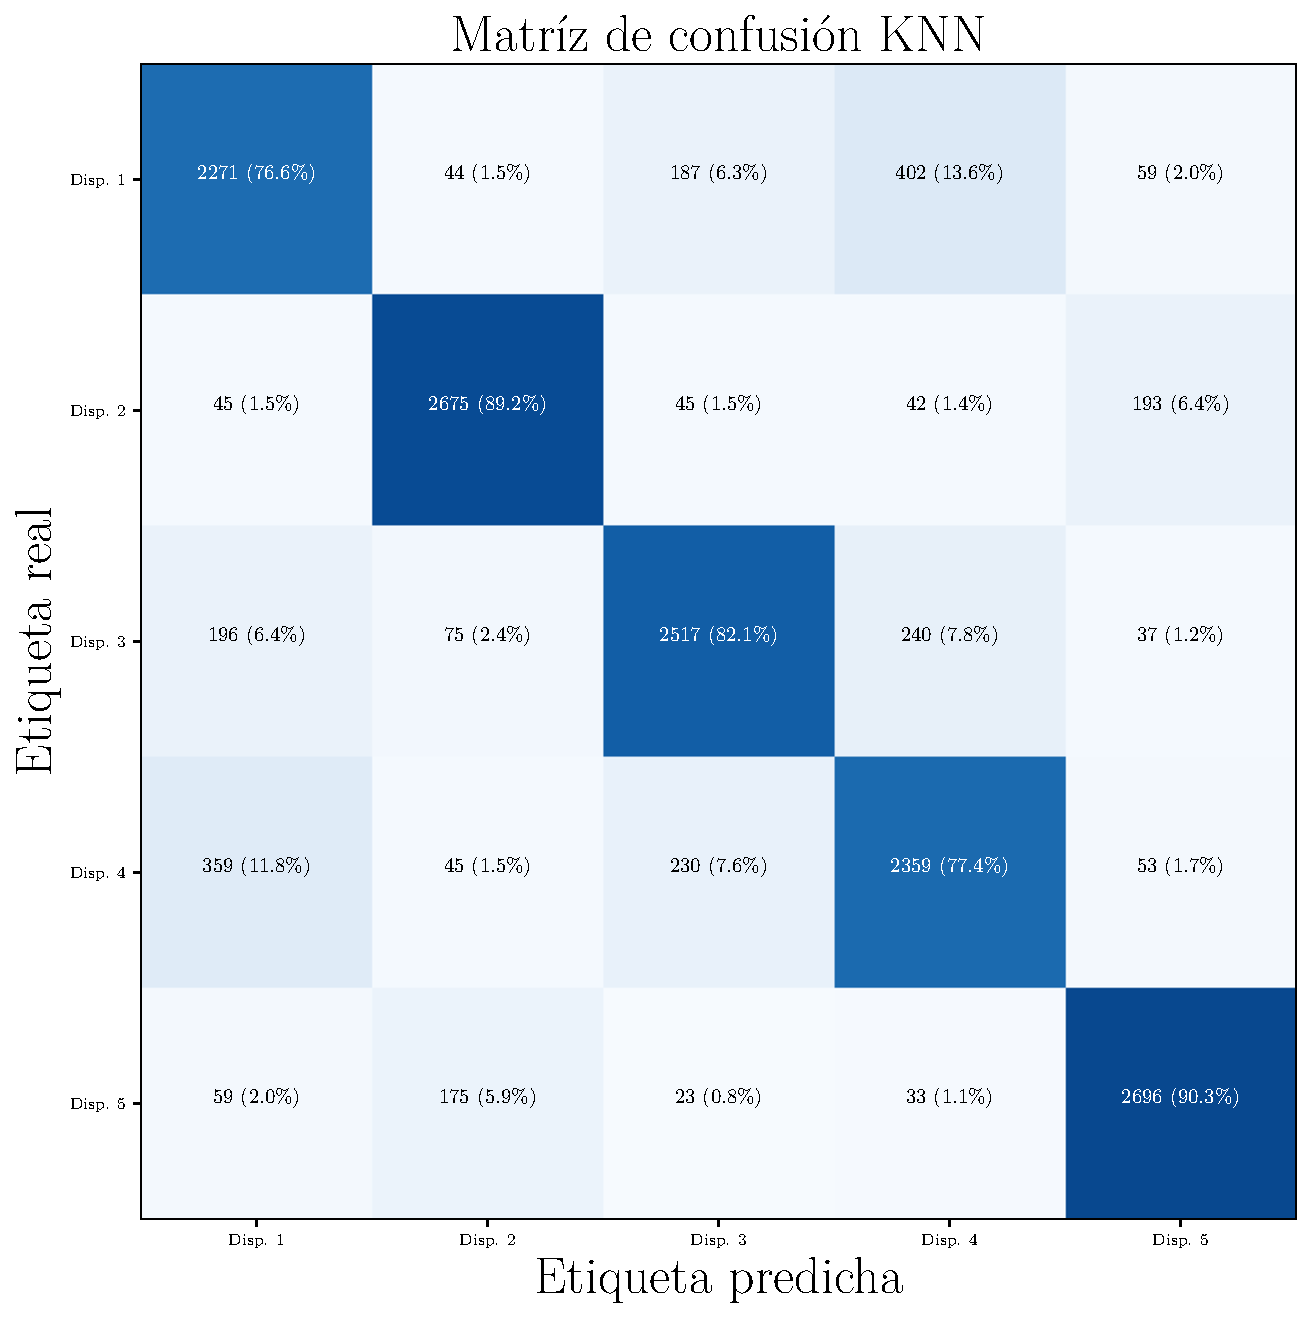
\includegraphics[width=0.4\textwidth]{../Python/plots/parallel/knn_matrix}} & \subfloat{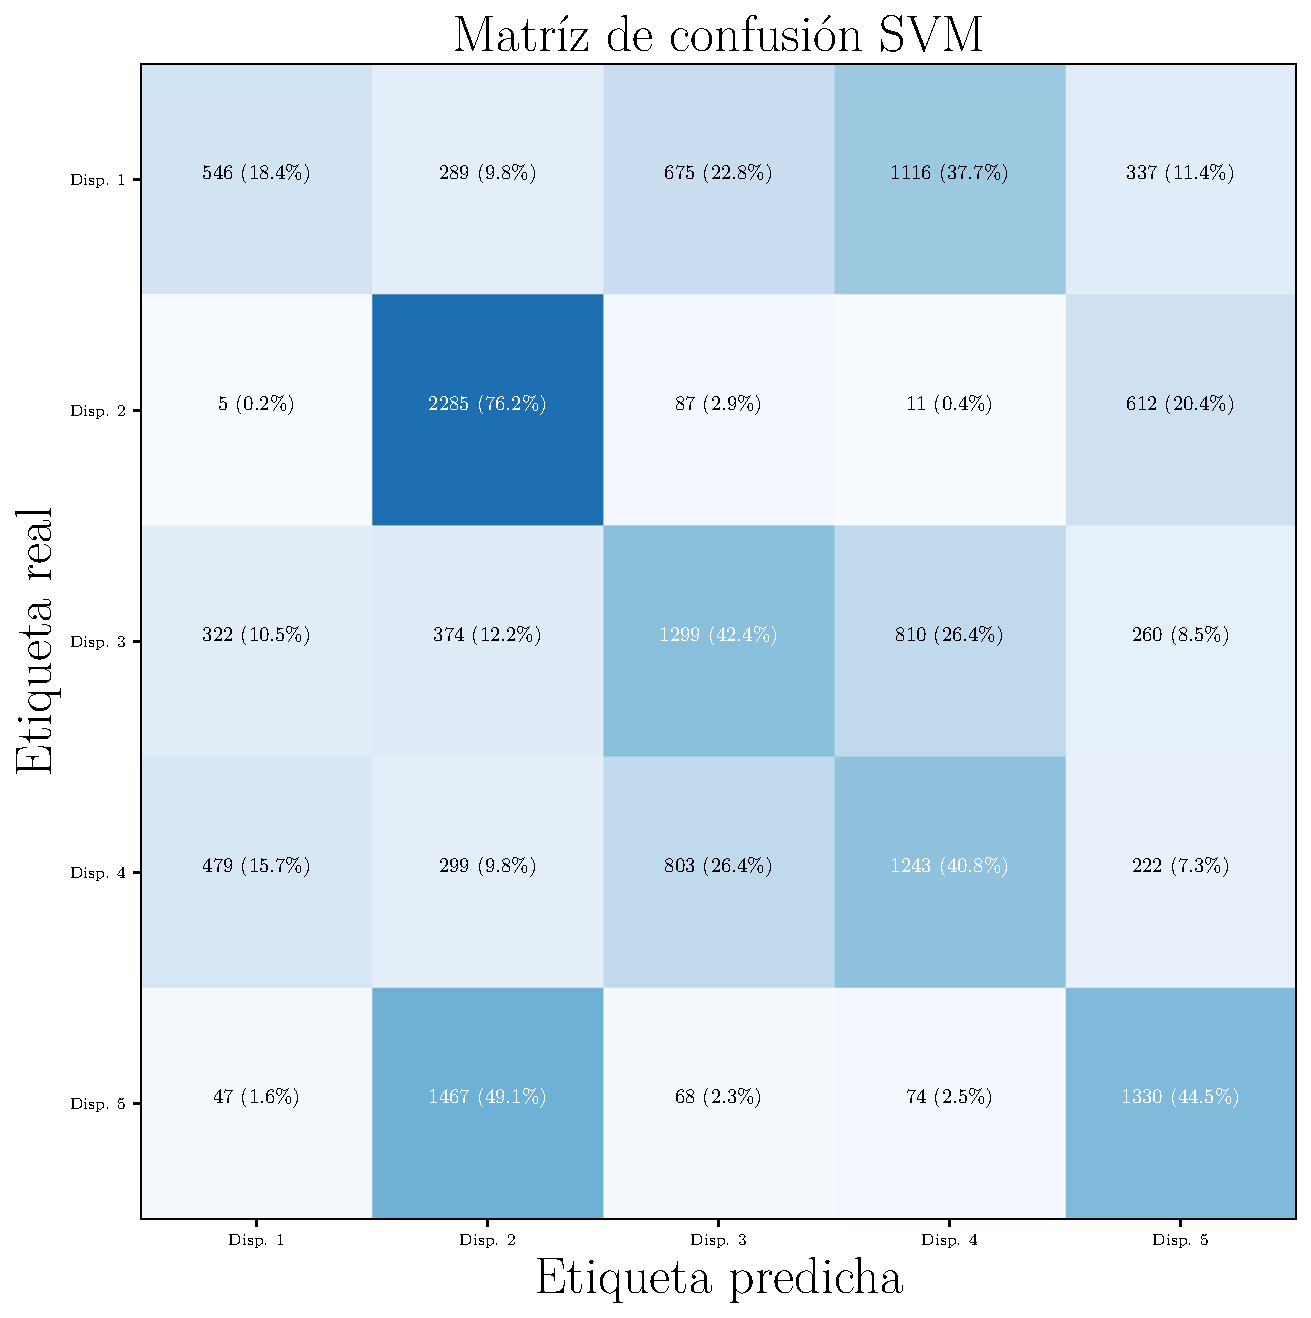
\includegraphics[width=0.4\textwidth]{../Python/plots/parallel/svm_linear_matrix}} & \\
    \end{tabular}
    \caption{Matrices de confusión con datos de la muestra paralela}
    \label{fig:confusion_matrices_parallel}
\end{figure}

Es fácil ver en la Fig. \ref{fig:confusion_matrices_parallel} que los modelos basados en árboles aciertan prácticamente en la totalidad de las ocasiones, en particular, el algoritmo de random forest es el que mejores resultados consigue ($\sim 99.5\%$). Por esta razón entrenaremos un modelo de random forest con los hiperparámetros ajustados anteriormente con la totalidad de los datos de entrenamiento. Los resultados obtenidos se pueden ver en la matriz de confusión resultante (Fig. \ref{fig:final_matrix}). Con estos resultados obtenemos un valor final de accuracy de 0.9944 (99.44\%).

\begin{figure}[H]
    \centering
    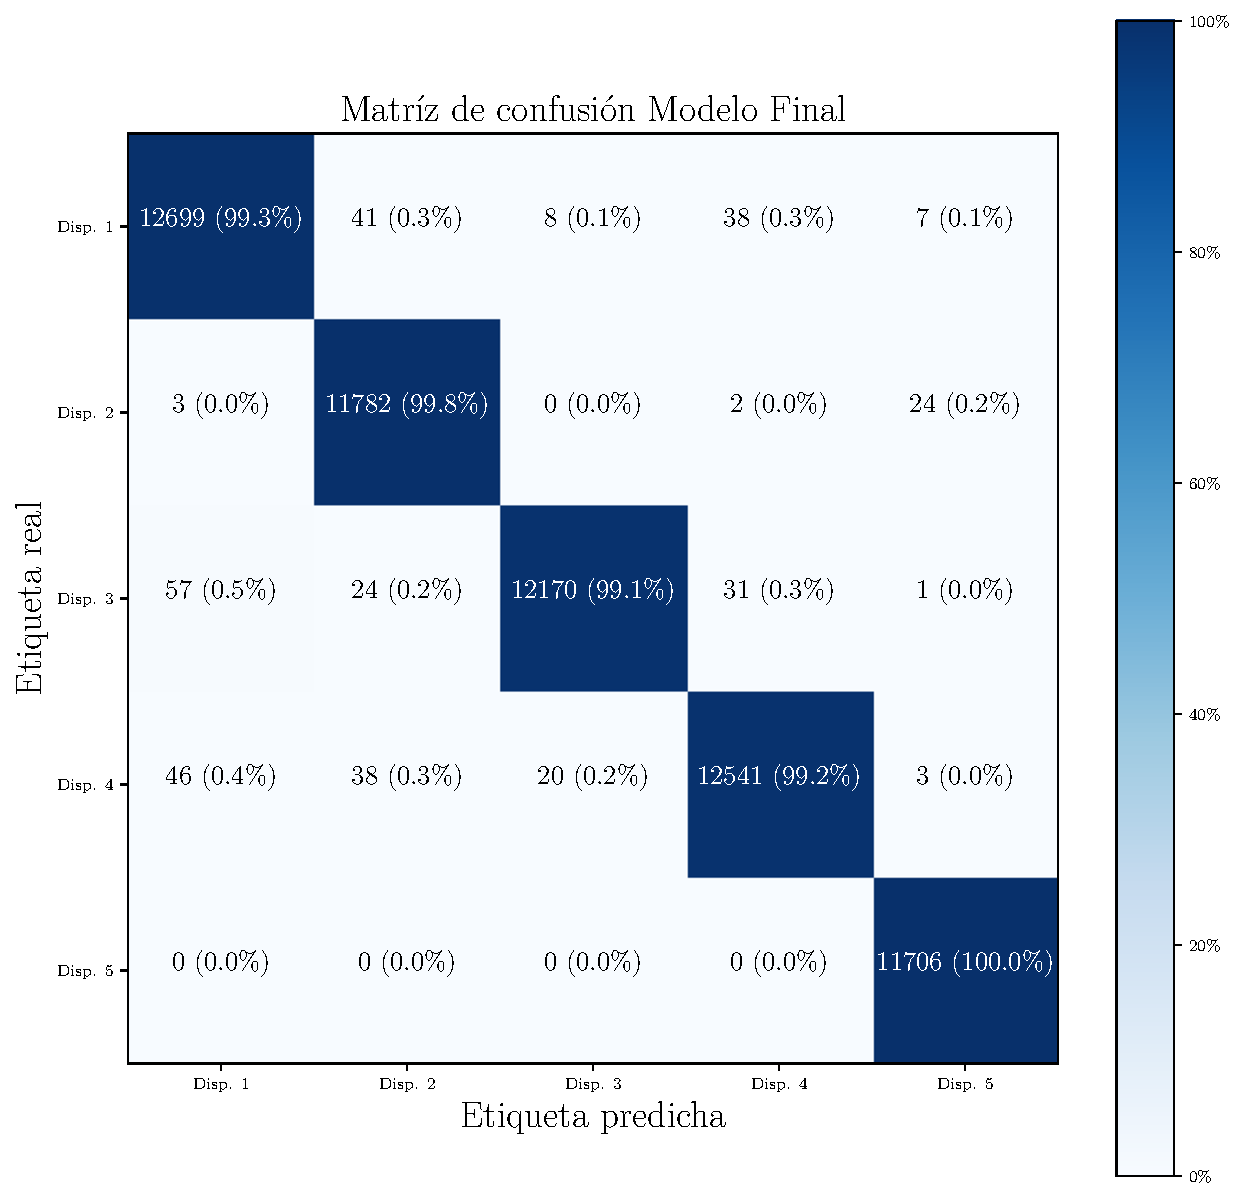
\includegraphics[scale=0.3]{../Python/plots/parallel/final_model_matrix}
    \caption{Matríz de confusión del modelo final}
    \label{fig:final_matrix}
\end{figure}

